\chapter{Thực nghiệm và đánh giá}
\label{chap:experiment}

\section{Môi trường thực nghiệm}
Các thí nghiệm được thực hiện trên một máy tính sử dụng bộ xử lý Intel Core i5-12450HX, có kiến trúc kết hợp nhân hiệu năng cao và nhân tiết kiệm điện. Bảng~\ref{tab:environment} trình bày cấu hình phần cứng, phần mềm và các tham số đo. Những thông số không được ghi nhận đầy đủ trong các đợt đo được chú thích riêng để tránh suy diễn.

\begin{table}[!htbp]
\centering\small
\caption{Phần cứng, phần mềm và tham số của phép đo}
\label{tab:environment}
\begin{tabularx}{\textwidth}{@{}p{.28\textwidth}Y@{}}
\toprule
Thành phần & Cấu hình \\
\midrule
CPU & Intel Core i5-12450HX \\
Nhân và luồng logic & 8 nhân, 12 luồng logic. Theo đặc tả \href{https://www.intel.com/content/www/us/en/products/sku/228794/}{Intel}, CPU có 4 P-core và 4 E-core. \\
Bộ nhớ đệm & Intel công bố \num{12} MB Smart Cache; chưa đối chiếu độc lập tổng dung lượng L2. \\
RAM & Hệ điều hành nhận \num{23.71} GiB. Dung lượng lắp đặt và số kênh chưa xác minh được. \\
Hệ điều hành & Windows 11. 26H2, build 26300.9974. \\
Trình biên dịch & GCC 16.2.0, MSYS2 UCRT64 \\
Cờ biên dịch & \texttt{-O2 -std=c11 -Wall -Wextra -Werror -fopenmp}; nhóm B và khảo sát số luồng thêm \texttt{-Wpedantic} \\
Thư viện OpenMP & libgomp UCRT64 16.2.0-6 (xác minh sau phép đo nhóm B); nhóm A không lưu phiên bản gói. \\
Số luồng so sánh chính & Serial 1 luồng. Basic và Optimized 8 luồng \\
Chính sách lập lịch & \texttt{static}. Chương trình tắt tự điều chỉnh số luồng \\
Gắn luồng, chế độ chờ & Nhóm A không ghi nhận; nhóm B và khảo sát số luồng dùng mặc định của runtime. Chưa đo vị trí luồng. \\
Chế độ nguồn, tải nền & Nhóm B và khảo sát số luồng dùng Balanced, có cắm điện khi lấy mẫu. Nhóm A không ghi nhận. \\
Bộ đếm thời gian & \texttt{QueryPerformanceCounter} trên Windows \\
Số lượt mỗi cấu hình & 2 lượt khởi động và 12 mẫu chính thức \\
\bottomrule
\end{tabularx}
\end{table}

\section{Bộ dữ liệu thực nghiệm}
\label{sec:datasets}
\subsection{Chu trình, lưới, thang và cây}
Để đánh giá ảnh hưởng của độ sâu, bề rộng tầng và quy mô đầu vào, nhóm sử dụng 12 đồ thị tổng hợp. Bộ dữ liệu được chia thành hai nhóm theo cách xây dựng và giao thức đo: nhóm A gồm chu trình, lưới, thang và ba cây; nhóm B gồm đường đi, sao, hai lưới rời, vòng có cung ngẫu nhiên và hai đồ thị phân tầng. Việc phân nhóm giúp đối chiếu đúng các phép đo có cùng giao thức. Sáu đồ thị có hướng thuộc nhóm A được sinh trong bộ nhớ và chuyển sang CSR. Từ nguồn $s=0$, BFS đi tới mọi đỉnh trong các đầu vào này. Độ sâu $D$ trong Bảng~\ref{tab:graphs} là khoảng cách lớn nhất tính từ nguồn. Số tầng chứa đỉnh là $L=D+1$ và bề rộng trung bình là $n/L$. Bề rộng cực đại lấy trực tiếp từ các công thức của từng cấu trúc.

\begin{table}[!htbp]
\centering\footnotesize
\setlength{\tabcolsep}{3pt}
\caption[Đặc trưng sáu đồ thị]{Đặc trưng của sáu đồ thị có hướng từ nguồn $s=0$. Số trong ngoặc là hạt giống xáo nhãn.}
\label{tab:graphs}
\begin{tabular}{@{}l S[table-format=8.0] S[table-format=8.0] S[table-format=4.0]
 S[table-format=4.0] S[table-format=6.2] S[table-format=7.0] l@{}}
\toprule
 & & & & & \multicolumn{2}{c}{Bề rộng (đỉnh)} & \\
\cmidrule(lr){6-7}
Đồ thị & {Số đỉnh} & {Số cung} & {$D$} & {$L$} & {T.bình} & {Lớn nhất} & Nhãn đỉnh \\
\midrule
% Generated by scripts/analysis/summarize.py
Chu trình & 2048 & 2048 & 2047 & 2048 & 1.00 & 1 & Theo cấu trúc \\
Thang & 2048 & 3070 & 1024 & 1025 & 2.00 & 2 & Theo cấu trúc \\
Lưới & 6144 & 12128 & 158 & 159 & 38.64 & 64 & Theo cấu trúc \\
Cây bậc ba nhỏ & 29524 & 29523 & 9 & 10 & 2952.40 & 19683 & Xáo (71) \\
Cây nhị phân lớn & 16777215 & 16777214 & 23 & 24 & 699050.63 & 8388608 & Xáo (2026) \\
Cây bậc bốn lớn & 5592405 & 5592404 & 11 & 12 & 466033.75 & 4194304 & Xáo (83) \\
\bottomrule

\end{tabular}
\end{table}

Chu trình có cung $v\to(v+1)\bmod n$ nên mỗi tầng có một đỉnh. Đồ thị thang có hai hàng, mỗi hàng có \num{1024} cột. Các cung dọc theo hàng đi sang phải, còn các cung giữa hai hàng chỉ đi từ hàng trên xuống hàng dưới tại cùng cột. Lưới có 64 hàng và 96 cột, với các cung đi sang phải hoặc xuống dưới. Các cây đầy đủ có cung từ cha xuống con, trong đó một đỉnh ở tầng $k$ đi tới $b$ đỉnh con nếu chưa phải lá.

Hai nhóm sơ đồ ở Hình~\ref{fig:graph-structures} và Hình~\ref{fig:graph-structures-new} minh họa quy tắc nối đỉnh trên mẫu thu nhỏ. Vòng tròn rỗng đánh dấu nguồn.

\begin{figure}[!htbp]
\centering
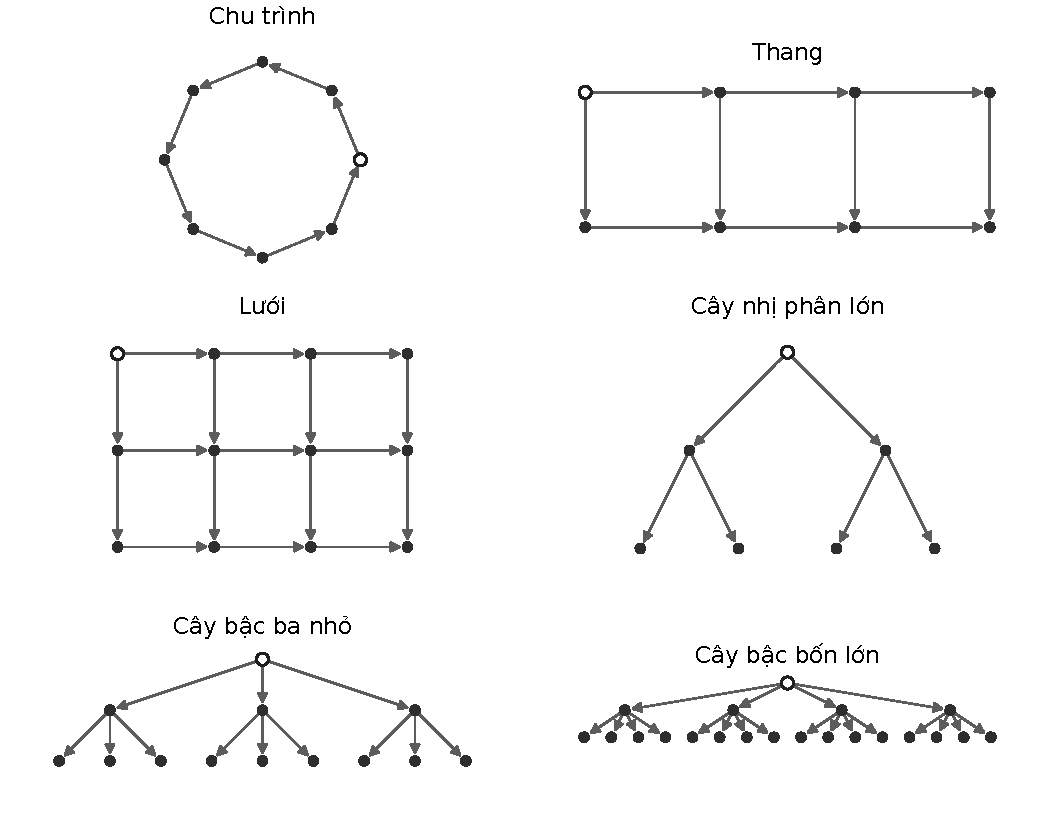
\includegraphics[width=.96\textwidth]{figures/graph-structures-24.pdf}
\caption[Cấu trúc chu trình, lưới, thang và cây]{Minh họa sáu cấu trúc đồ thị thuộc nhóm A. Mũi tên biểu thị hướng cung.}
\label{fig:graph-structures}
\end{figure}

\subsection{Bề rộng tầng và cách đánh số}
Trên thang, tầng nguồn và tầng cuối đều có một đỉnh, các tầng ở giữa có hai đỉnh. Trên lưới, khoảng cách của ô $(r,c)$ bằng $r+c$. Số ô ở tầng $k$ bằng
\[
 \min(63,k)-\max(0,k-95)+1,\qquad 0\le k\le158.
\]
Trên cây bậc $b$, tầng $k$ chứa đúng $b^k$ đỉnh. Hình~\ref{fig:width} dùng số đỉnh tính theo các quy tắc này.

\experimentfig{layer-width}{Bề rộng tầng của sáu đồ thị}
{Số đỉnh ở từng tầng của sáu đồ thị, tính từ quy tắc dựng đồ thị trong bộ sinh. Trục tung dùng thang logarit. Các giá trị biểu diễn cấu trúc tổ hợp, không phải số đo thời gian.}
{fig:width}
{Hình~\ref{fig:width} phân biệt hai kiểu hình dạng tầng. Chu trình và thang giữ bề rộng gần như cố định. Lưới có bề rộng tăng, giữ ổn định rồi giảm theo đường chéo. Trên các cây, bề rộng tăng theo cấp số nhân; các tầng đầu hẹp, trong khi hai tầng cuối chiếm phần lớn số đỉnh.}

Chu trình giữ nhãn theo thứ tự dọc chu trình, nên khoảng cách bằng nhãn. Thang đánh nhãn lần lượt theo từng cột, lưới theo từng hàng. Khoảng cách trên thang và lưới được tính từ tọa độ, vì vậy thường khác nhãn số. Với các cây, bộ sinh xáo nhãn của các đỉnh khác gốc theo hạt giống cố định, giữ gốc bằng $0$. Việc xáo nhãn giữ nguyên các quan hệ cha con và bề rộng tầng, nhưng thay vị trí của các đỉnh trong các mảng được lập chỉ số bằng nhãn.

\subsection{Đường đi, sao và các đồ thị có cấu trúc mở rộng}
Nhóm B được xây dựng nhằm khảo sát sự khác biệt giữa bề rộng tầng và lượng công việc thực tế. Đường đi có nhiều tầng hẹp; đồ thị sao có một đỉnh bậc ra lớn; hai lưới vô hướng tách rời kiểm tra khả năng xử lý đồ thị không liên thông. Ba đồ thị còn lại cung cấp nhiều cung hơn cho các tầng có nhiều đỉnh. \texttt{ring-random} ghép một vòng có hướng với sáu cung ngẫu nhiên phân biệt đi ra từ mỗi đỉnh. Hai đồ thị phân tầng xáo nhãn đỉnh. \texttt{layered-overlap} tập trung nhiều cung vào một nhóm nhỏ đỉnh ở tầng kế tiếp, còn \texttt{layered-permuted} dùng các phép dịch vòng để phân bố cung đều hơn. Quy tắc sinh, kích thước và hạt giống được xác định trước khi tiến hành đo để bảo đảm khả năng tái lập. Do không tải được dữ liệu SNAP trong môi trường thực nghiệm, phạm vi khảo sát được giới hạn ở các đồ thị tổng hợp. Các nghiên cứu chuẩn hóa benchmark như GAP cung cấp tiền lệ cho việc công bố cả quy tắc đầu vào và phương pháp đánh giá \cite{gap2015}.

Bảng~\ref{tab:supplement-graphs} dùng $m_{\mathrm{in}}$ cho số liên kết đầu vào. Hai lưới rời có \num{65024} cạnh và \num{130048} cung trong CSR. Từ nguồn, BFS tới \num{16384} đỉnh và xét \num{65024} cung. Trên đồ thị có hướng, mỗi liên kết đầu vào là một cung. Hạt giống của vòng có cung ngẫu nhiên, phân tầng hội tụ và phân tầng hoán vị lần lượt là \num{34178}, \num{39014} và \num{46029}.

\begin{table}[!htbp]
\centering\footnotesize
\setlength{\tabcolsep}{3pt}
\caption{Đặc trưng của sáu đồ thị nhóm B với nguồn $s=0$}
\label{tab:supplement-graphs}
\begin{tabular}{@{}ll S[table-format=7.0] S[table-format=7.0] S[table-format=7.0]
S[table-format=3.0] S[table-format=6.0]@{}}
\toprule
Đồ thị & Hướng & {$n$} & {$m_{\mathrm{in}}$} & {Tới được} & {Tầng} & {Rộng nhất} \\
\midrule
Đường đi & Có hướng & 513 & 512 & 513 & 513 & 1 \\
Sao & Có hướng & 262144 & 262143 & 262144 & 2 & 262143 \\
Hai lưới rời & Vô hướng & 32768 & 65024 & 16384 & 255 & 128 \\
Vòng có cung ngẫu nhiên & Có hướng & 350000 & 2450000 & 350000 & 11 & 203533 \\
Phân tầng hội tụ & Có hướng & 393217 & 5799936 & 393217 & 13 & 32768 \\
Phân tầng hoán vị & Có hướng & 1048577 & 7929856 & 1048577 & 17 & 65536 \\
\bottomrule

\end{tabular}
\end{table}


\begin{figure}[!htbp]
\centering
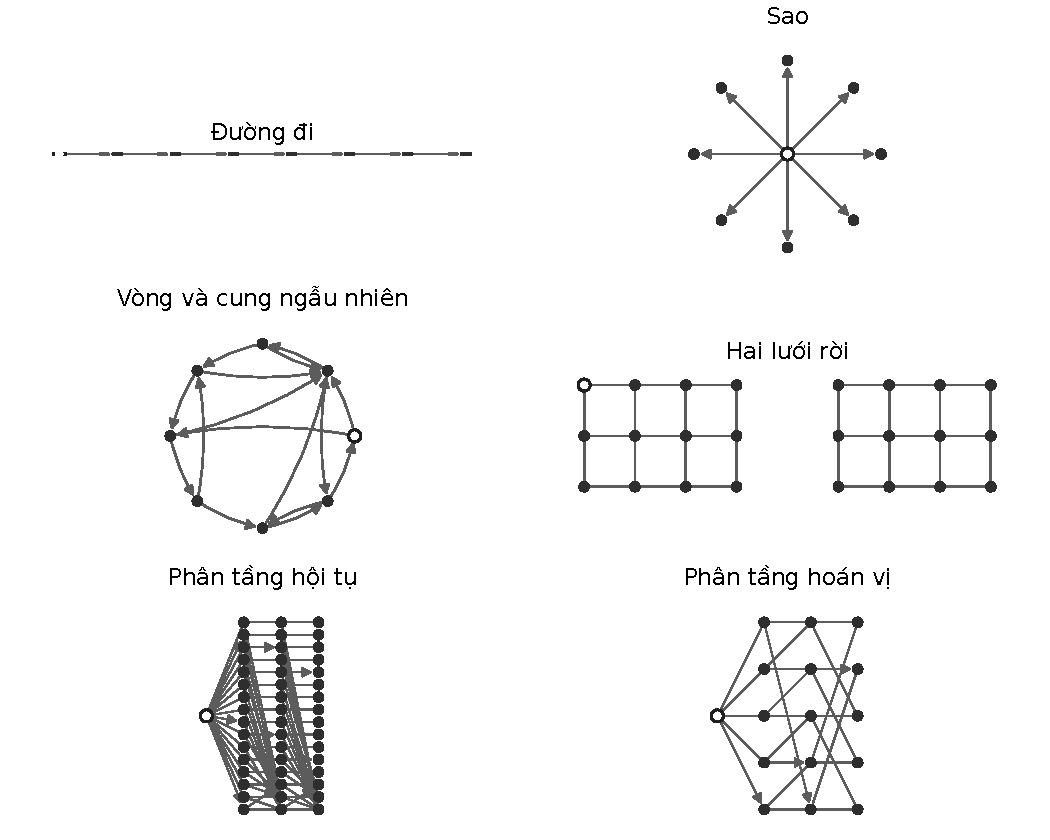
\includegraphics[width=.96\textwidth]{figures/graph-structures-25.pdf}
\caption[Cấu trúc các đồ thị nhóm B]{Minh họa sáu cấu trúc đồ thị thuộc nhóm B. Hai lưới rời là vô hướng; mũi tên trong hai mẫu phân tầng biểu thị một số cung đại diện theo chiều từ trái sang phải.}
\label{fig:graph-structures-new}
\end{figure}

\section{Phương pháp thực nghiệm}
\label{sec:measurement}
\subsection{Kiểm chứng khoảng cách}
Đối với nhóm A, chương trình xác định khoảng cách tham chiếu từ quy tắc xây dựng đồ thị. Khoảng cách tới hai nút ở cột $j$ của thang là $j$ và $j+1$. Lưới dùng $r+c$, còn cây dùng độ sâu của đỉnh trong cấu trúc trước khi xáo nhãn. Mảng đối chiếu của cây được ghi theo nhãn đã xáo để so trực tiếp với đầu ra BFS. Sau mỗi lời gọi, chương trình chỉ ghi mẫu khi hàm trả trạng thái thành công, số luồng đúng yêu cầu và toàn bộ mảng khoảng cách trùng với đáp án.

Đối với nhóm B và khảo sát số luồng, chương trình so sánh từng phần tử khoảng cách với kết quả của một cài đặt BFS tham chiếu độc lập trên cùng CSR. Kiểm chứng này bao phủ đầu ra duyệt, còn việc tạo CSR có các kiểm thử parser riêng. Trình đo xác thực cả số luồng thực thi và trạng thái trả về.

\subsection{Phạm vi đo và thống kê}
Với mỗi đồ thị, chương trình dựng CSR một lần rồi dùng lại trong một tiến trình. Mỗi vòng gọi ba thuật toán theo thứ tự xoay vòng. Hai vòng đầu mang chỉ số $-2,-1$ và làm nhiệm vụ khởi động. Mười hai vòng tiếp theo mang chỉ số $0$ đến $11$. Do thứ tự luân phiên theo chu kỳ ba, mỗi thuật toán đứng ở mỗi vị trí đúng bốn lần trong 12 vòng chính thức. Mỗi nhóm có 252 lượt đo hợp lệ, trong đó 216 mẫu chính thức được sử dụng để tính thống kê.

Chương trình gọi bộ đếm thời gian Windows ngay trước và sau hàm BFS.\footnote{Xem \href{https://learn.microsoft.com/en-us/windows/win32/api/profileapi/nf-profileapi-queryperformancecounter}{tài liệu QueryPerformanceCounter của Microsoft}.} Khoảng đo bao gồm các thao tác trong hàm, kể cả khởi tạo khoảng cách, cấp phát và giải phóng vùng đệm. Việc dựng CSR, cấp phát mảng đầu ra của phía gọi, kiểm tra khoảng cách và ghi CSV nằm ngoài khoảng đo. Nhóm tính các chỉ số theo Mục~\ref{sec:metrics} từ mẫu chính thức, giữ nguyên các quan sát và thứ tự vòng.

Thực nghiệm so sánh ba phiên bản có tổng cộng 504 lượt, gồm 72 lượt khởi động và 432 mẫu chính thức. Nhóm A tạo CSR trực tiếp từ danh sách cung trong bộ nhớ; nhóm B đọc danh sách liên kết từ tệp và lưu thêm số luồng yêu cầu, số luồng thực tế và hồ sơ các tầng. Cả hai nhóm sử dụng nguồn $0$, lịch tĩnh và cùng số lần lặp. Tần số bộ đếm QPC ghi nhận khi đo nhóm B là \num{10000000} Hz. Do các nhóm được đo ở những thời điểm khác nhau, mọi hệ số tăng tốc đều sử dụng thời gian Serial đo trên cùng đồ thị và trong cùng đợt thực nghiệm. Thông tin về thời điểm đo và cách tái lập được lưu trong Phụ lục~\ref{app:reproduce}.

\section{Kết quả thực nghiệm}
\label{sec:results}
\subsection{So sánh hiệu năng trên chu trình, lưới, thang và cây}
Các biểu đồ thời gian thực thi và hệ số tăng tốc được xây dựng từ 12 mẫu chính thức của mỗi cấu hình. Nhóm sử dụng trung vị để so sánh thời gian điển hình và khoảng tứ phân vị để biểu diễn độ phân tán của các phép đo.
Bảng~\ref{tab:results} gộp thời gian, hệ số tăng tốc và hiệu suất. Giá trị trung vị thấp nhất trên mỗi đồ thị được in đậm. Cột cuối dùng $1/S_8$ khi OpenMP mất nhiều thời gian hơn Serial. Phụ lục~\ref{app:quartiles} cung cấp các tứ phân vị riêng, độ rộng khoảng tứ phân vị và hai cực trị.

\begin{table}[!htbp]
\centering\footnotesize
\setlength{\tabcolsep}{3pt}
\caption[Thời gian, hệ số tăng tốc và hiệu suất]{Kết quả từ 12 mẫu mỗi cấu hình. Khoảng thời gian viết dưới dạng $[Q_1;Q_3]$.}
\label{tab:results}
\begin{tabular}{@{}ll S[table-format=4.4] c S[table-format=1.4e-1]
 S[table-format=2.4] S[table-format=5.2]@{}}
\toprule
Đồ thị & Bản BFS & {Trung vị (ms)} & {$[Q_1;Q_3]$ (ms)} & {$S_8$} & {$E_8$ (\%)} & {Chậm hơn} \\
 & & & & & & {Serial (lần)} \\
\midrule
% Generated by scripts/analysis/summarize.py
Chu trình & Serial & \bfseries 0.0105 & [\num{0.0100}\,\textup{;}\,\num{0.0106}] & {} & {} & {} \\
 & Basic & 321.5206 & [\num{293.7409}\,\textup{;}\,\num{370.4228}] & 3.25e-5 & 0.0004 & 30767.52 \\
 & Optimized & 516.1245 & [\num{496.3574}\,\textup{;}\,\num{652.1391}] & 2.02e-5 & 0.0003 & 49389.90 \\
Thang & Serial & \bfseries 0.0162 & [\num{0.0154}\,\textup{;}\,\num{0.0170}] & {} & {} & {} \\
 & Basic & 136.3073 & [\num{133.9077}\,\textup{;}\,\num{153.4679}] & 1.18e-4 & 0.0015 & 8440.08 \\
 & Optimized & 231.4461 & [\num{223.7024}\,\textup{;}\,\num{250.6293}] & 6.98e-5 & 0.0009 & 14331.02 \\
Lưới & Serial & \bfseries 0.0357 & [\num{0.0338}\,\textup{;}\,\num{0.0363}] & {} & {} & {} \\
 & Basic & 21.5734 & [\num{20.7224}\,\textup{;}\,\num{22.2761}] & 1.65e-3 & 0.0207 & 604.30 \\
 & Optimized & 36.0463 & [\num{34.1242}\,\textup{;}\,\num{37.1938}] & 9.90e-4 & 0.0124 & 1009.70 \\
Cây bậc ba nhỏ & Serial & \bfseries 0.0952 & [\num{0.0852}\,\textup{;}\,\num{0.1047}] & {} & {} & {} \\
 & Basic & 2.8444 & [\num{2.6924}\,\textup{;}\,\num{3.0311}] & 0.0335 & 0.4181 & 29.89 \\
 & Optimized & 3.2873 & [\num{3.2391}\,\textup{;}\,\num{3.4055}] & 0.0289 & 0.3618 & 34.55 \\
Cây nhị phân lớn & Serial & 1169.4313 & [\num{596.4765}\,\textup{;}\,\num{1281.2918}] & {} & {} & {} \\
 & Basic & 765.4273 & [\num{704.0538}\,\textup{;}\,\num{805.2672}] & 1.5278 & 19.0977 & {} \\
 & Optimized & \bfseries 496.7922 & [\num{471.3353}\,\textup{;}\,\num{506.2669}] & 2.3540 & 29.4246 & {} \\
Cây bậc bốn lớn & Serial & 163.6414 & [\num{161.2972}\,\textup{;}\,\num{169.0367}] & {} & {} & {} \\
 & Basic & 214.8783 & [\num{213.6967}\,\textup{;}\,\num{217.2856}] & 0.7616 & 9.5194 & 1.31 \\
 & Optimized & \bfseries 130.3665 & [\num{121.4354}\,\textup{;}\,\num{140.9594}] & 1.2552 & 15.6905 & {} \\
\bottomrule

\end{tabular}
\end{table}

\experimentfig{time-iqr}{Thời gian trung vị và khoảng tứ phân vị}
{Trung vị thời gian theo đồ thị và phiên bản, tính bằng ms. Trục tung dùng thang logarit. Mỗi điểm dùng 12 mẫu chính thức, với thanh từ $Q_1$ đến $Q_3$.}
{fig:runtime}
{Hình~\ref{fig:runtime} cho thấy thời gian ba phiên bản khác nhau nhiều bậc trên chu trình, thang và lưới. Trên hai cây lớn, khoảng tứ phân vị của Optimized nằm hoàn toàn dưới khoảng tứ phân vị của Serial. Cây nhị phân lớn có khoảng tứ phân vị Serial rộng hơn nhiều so với các cấu hình còn lại trên cùng đồ thị (Bảng~\ref{tab:results}).}

\experimentfig{speedup}{Hệ số tăng tốc với tám luồng}
{Hệ số $S_8$ của Basic và Optimized, lấy tỷ số trung vị từ 12 mẫu mỗi phiên bản. Trục tung dùng thang logarit. Đường đứt tại $S_8=1$ biểu thị trung vị bằng Serial.}
{fig:speedup}
{Ba trong 12 điểm của Hình~\ref{fig:speedup} vượt mốc $1$. Basic vượt mốc trên cây nhị phân lớn, Optimized vượt mốc trên cả hai cây lớn. Trên chu trình, hệ số của Basic khoảng $\num{3.3e-5}$ (Bảng~\ref{tab:results}).}

\subsection{So sánh hiệu năng trên đường đi, sao và đồ thị nhiều cung}
Bảng~\ref{tab:supplement-results} ghi trung vị từng phiên bản và hệ số của Optimized so với Serial. Hình~\ref{fig:supplement-performance} bổ sung khoảng từ $Q_1$ đến $Q_3$ và hệ số của cả hai bản OpenMP. Hình~\ref{fig:supplement-frontier} thể hiện vị trí và độ rộng của các tầng.

\begin{table}[!htbp]
\centering\footnotesize
\setlength{\tabcolsep}{3pt}
\caption{Thời gian trung vị (ms), hệ số tăng tốc và hiệu suất trên nhóm B}
\label{tab:supplement-results}
\begin{tabular}{@{}l *{3}{S[table-format=3.5]} S[table-format=1.5e-1]
S[table-format=2.6] @{\hspace{6pt}}l@{}}
\toprule
Đồ thị & {Serial} & {Basic} & {Optimized} & {$S_8$} & {$E_8$ (\%)} & Nhanh nhất \\
\midrule
Đường đi & 0.0048 & 105.218 & 174.767 & 2.75e-05 & 0.000343 & Serial \\
Sao & 0.70505 & 3.85805 & 3.28985 & 0.214 & 2.68 & Serial \\
Hai lưới rời & 0.1293 & 60.8294 & 104.869 & 0.00123 & 0.0154 & Serial \\
Vòng có cung ngẫu nhiên & 22.7852 & 25.0149 & 19.487 & 1.17 & 14.6 & Optimized \\
Phân tầng hội tụ & 51.8015 & 48.431 & 37.5748 & 1.38 & 17.2 & Optimized \\
Phân tầng hoán vị & 151.158 & 85.3081 & 71.1679 & 2.12 & 26.5 & Optimized \\
\bottomrule

\end{tabular}
\end{table}

\begin{figure}[!htbp]
\centering
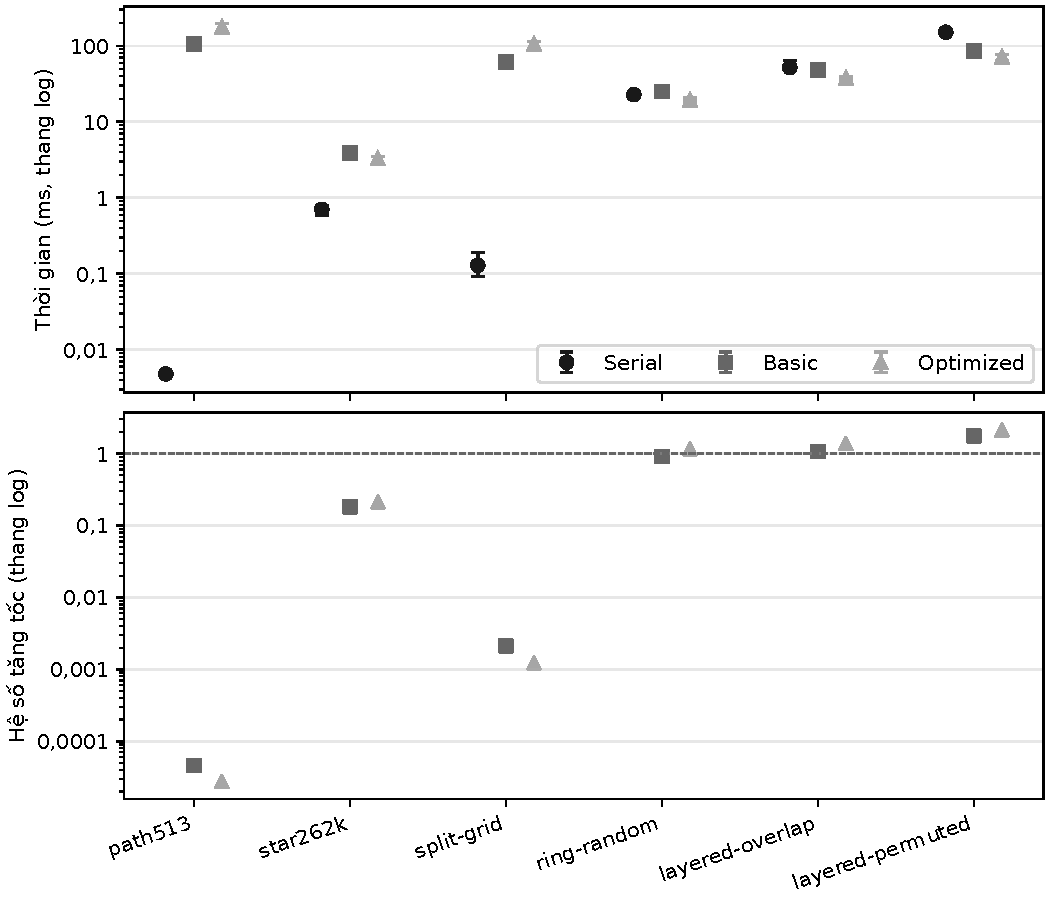
\includegraphics[width=.88\textwidth]{figures/supplement-performance.pdf}
\caption[Thời gian và hệ số tăng tốc trên nhóm B]{Thời gian trung vị, khoảng $[Q_1,Q_3]$ và hệ số tăng tốc của các phiên bản trên nhóm B. Hai trục tung sử dụng thang logarit.}
\label{fig:supplement-performance}
\end{figure}

\begin{figure}[!htbp]
\centering
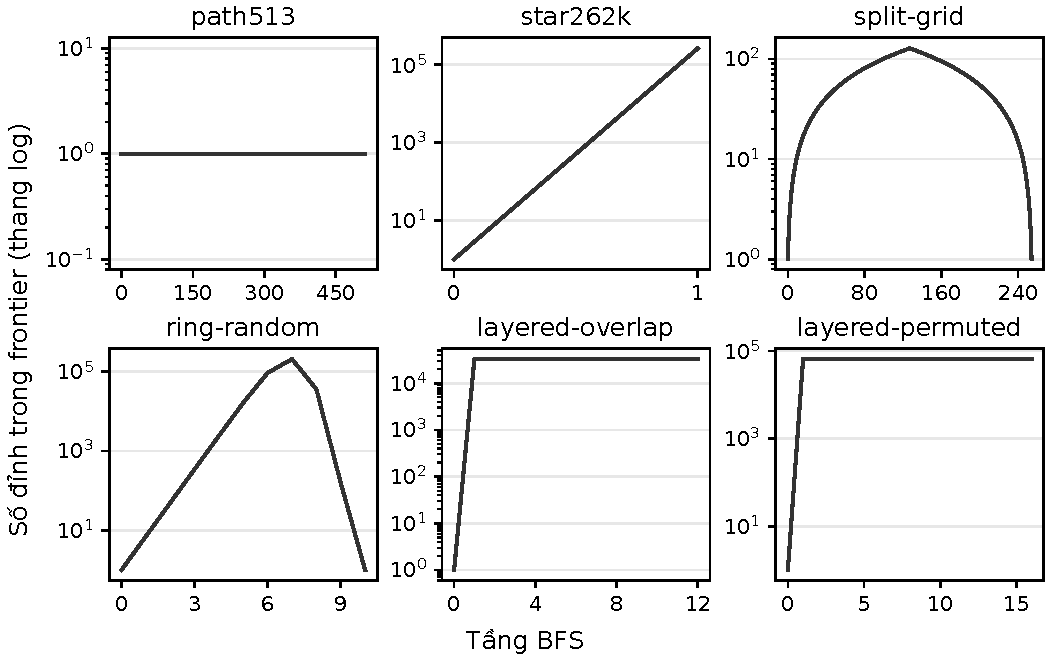
\includegraphics[width=.88\textwidth]{figures/supplement-frontier.pdf}
\caption[Bề rộng các tầng của đồ thị nhóm B]{Số đỉnh tại mỗi tầng BFS tính từ nguồn $s=0$ trên nhóm B. Trục bề rộng sử dụng thang logarit.}
\label{fig:supplement-frontier}
\end{figure}

\subsection{Tổng hợp và so sánh hiệu năng}
Bảng~\ref{tab:comparison} tổng hợp thời gian trung vị và hệ số tăng tốc của Optimized trên toàn bộ 12 đồ thị, phân theo hai nhóm dữ liệu. Serial đạt thời gian trung vị thấp nhất trên 7 đồ thị, Optimized trên 5 đồ thị. Basic không đạt trung vị thấp nhất trên đồ thị nào trong bộ dữ liệu này. Đây là kết quả trên 12 đầu vào cố định. Phụ lục~\ref{app:quartiles} lưu các thống kê phân tán của cả 36 cặp đồ thị--phiên bản.

\begin{table}[!htbp]
\centering\footnotesize
\setlength{\tabcolsep}{3.5pt}
\caption{Đối chiếu trên 12 đồ thị, trung vị theo ms và $S_8$ của Optimized}
\label{tab:comparison}
\begin{tabular}{@{}l *{3}{S[table-format=4.5]} S[table-format=1.5e-1] l@{}}
\toprule
Đồ thị & {Serial} & {Basic} & {Optimized} & {$S_8$} & Nhanh nhất \\
\midrule
\textbf{Nhóm A} & {} & {} & {} & {} & {} \\
Chu trình & 0.01045 & 321.521 & 516.124 & 2.02e-05 & Serial \\
Lưới & 0.0357 & 21.5734 & 36.0463 & 0.00099 & Serial \\
Đồ thị thang & 0.01615 & 136.307 & 231.446 & 6.98e-05 & Serial \\
Cây bậc ba nhỏ & 0.09515 & 2.8444 & 3.2873 & 0.0289 & Serial \\
Cây nhị phân lớn & 1169.43 & 765.427 & 496.792 & 2.35 & Optimized \\
Cây bậc bốn lớn & 163.641 & 214.878 & 130.366 & 1.26 & Optimized \\
\midrule
\textbf{Nhóm B} & {} & {} & {} & {} & {} \\
Đường đi & 0.0048 & 105.218 & 174.767 & 2.75e-05 & Serial \\
Sao & 0.70505 & 3.85805 & 3.28985 & 0.214 & Serial \\
Hai lưới rời & 0.1293 & 60.8294 & 104.869 & 0.00123 & Serial \\
Vòng có cung ngẫu nhiên & 22.7852 & 25.0149 & 19.487 & 1.17 & Optimized \\
Phân tầng hội tụ & 51.8015 & 48.431 & 37.5748 & 1.38 & Optimized \\
Phân tầng hoán vị & 151.158 & 85.3081 & 71.1679 & 2.12 & Optimized \\
\bottomrule

\end{tabular}
\end{table}

\subsection{Khảo sát theo số luồng}
\label{sec:scaling}
Phiên riêng ngày 25/11 dùng lại đường đi, vòng có cung ngẫu nhiên và phân tầng hoán vị sau khi xác minh SHA-256 của danh sách cung và đối chiếu hồ sơ các tầng. Mỗi đồ thị có 11 cấu hình, gồm Serial một luồng và hai bản OpenMP với $p\in\{1,2,4,8,12\}$, lịch tĩnh. Thứ tự cấu hình xoay giữa các vòng. Phiên hoàn thành 66 lượt khởi động và 396 mẫu chính thức. Mỗi lượt đều được kiểm tra bằng mảng khoảng cách tham chiếu và số luồng thực tế. Mốc Serial được đo cùng phiên.

\begin{figure}[!htbp]
\centering
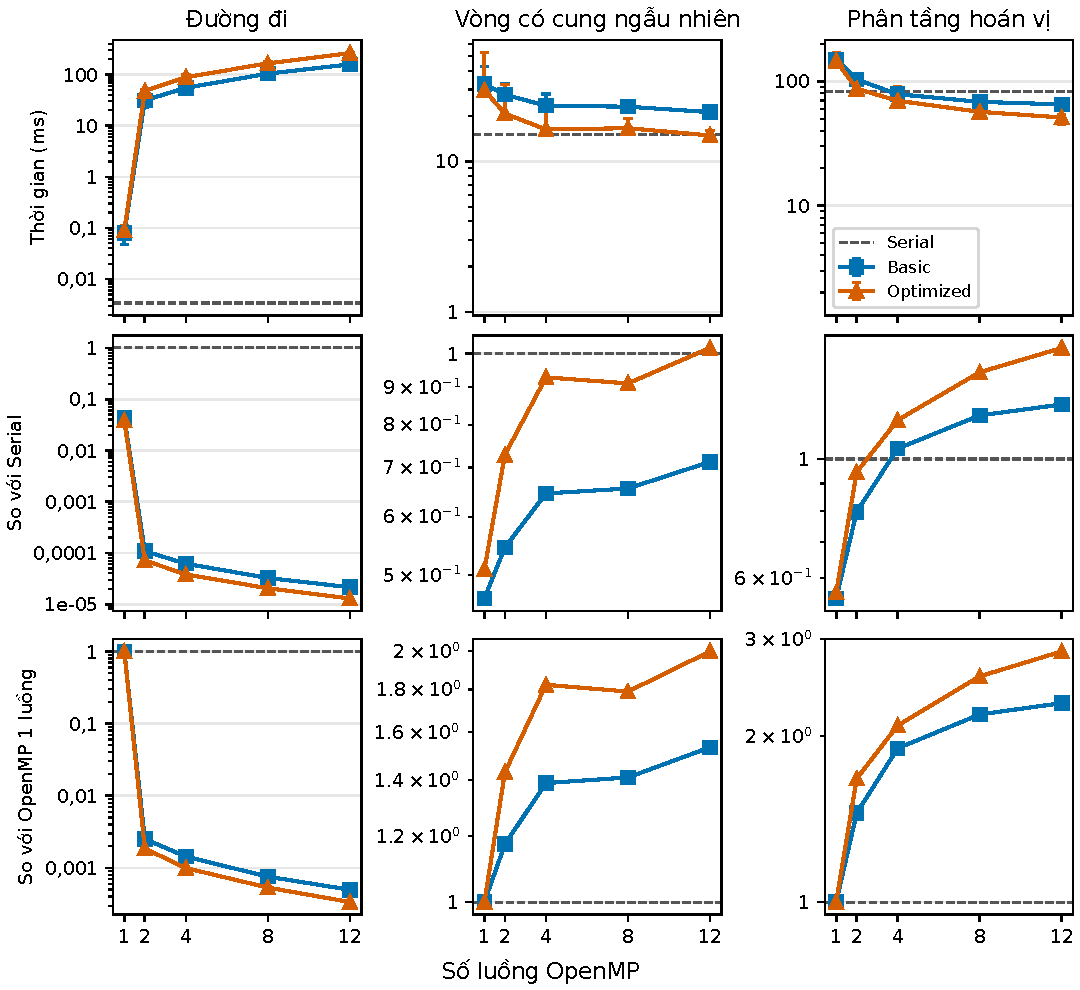
\includegraphics[width=.95\textwidth]{figures/thread-scaling.pdf}
\caption[Thời gian và hệ số theo số luồng]{Phiên khảo sát luồng với 12 mẫu chính thức mỗi cấu hình. Hàng trên là trung vị và khoảng $[Q_1,Q_3]$. Hai hàng dưới lần lượt dùng Serial và OpenMP một luồng làm mốc. Các trục đứng dùng thang logarit.}
\label{fig:scaling}
\end{figure}

Trên đường đi, Serial mất \num{0.0034} ms. Optimized tăng từ \num{0.0887} ms ở một luồng lên \num{166.23} ms ở tám luồng và \num{263.56} ms ở 12 luồng. Hai bản OpenMP đều chậm dần khi tăng số luồng. Kết quả này nhất quán với cấu trúc chỉ có một đỉnh mỗi tầng.

Vòng có cung ngẫu nhiên có trung vị Optimized \num{16.609} ms ở tám luồng và \num{14.863} ms ở 12 luồng, so với Serial \num{15.133} ms. Mức tăng tốc ở 12 luồng xấp xỉ \num{1.02}. Các khoảng tứ phân vị chồng lấn, vì vậy chênh lệch trung vị nhỏ cần được diễn giải thận trọng. Basic có trung vị thấp nhất ở 12 luồng trong các mức của chính Basic, nhưng vẫn chậm hơn Serial.

Phân tầng hoán vị cải thiện từ \num{56.797} ms ở tám luồng xuống \num{51.179} ms ở 12 luồng với Optimized. Ở 12 luồng, hệ số so với Serial là \num{1.61}, hiệu suất là \num{13.4}\%, và hệ số nội bộ so với Optimized một luồng là \num{2.85}. Hình~\ref{fig:scaling} và Phụ lục~\ref{app:scaling} ghi toàn bộ mức luồng. CPU có tám nhân vật lý, 12 luồng logic. Nhóm dùng cách bố trí luồng mặc định của hệ điều hành và runtime, vì vậy dữ liệu chưa cho biết tác động riêng của P-core, E-core hoặc SMT.


\section{Phân tích và thảo luận}
\subsection{Đồ thị hẹp và sâu}
Chu trình và thang có lần lượt \num{2048} và \num{1025} tầng, mỗi tầng chứa tối đa một hoặc hai đỉnh (Bảng~\ref{tab:graphs}). Vì vòng lặp chia việc theo đỉnh, phần lớn luồng không nhận đỉnh ở các tầng đó. Bảng~\ref{tab:results} cho thấy Basic mất khoảng \num{30768} lần thời gian của Serial trên chu trình và \num{8440} lần trên thang. Hai đồ thị có cùng số đỉnh nhưng khác số tầng và số cung. Trường hợp này phù hợp với giả thuyết rằng việc lặp qua nhiều rào có thể lấn át phần việc hữu ích.

Lưới có tối đa 64 đỉnh một tầng, nhưng Basic vẫn mất khoảng 604 lần thời gian của Serial. Cây bậc ba nhỏ cho một đối chiếu khác: chỉ có 10 tầng và đạt bề rộng cực đại \num{19683} đỉnh, song Basic vẫn mất khoảng 30 lần thời gian Serial (Bảng~\ref{tab:results}). Bề rộng cực đại cho biết tiềm năng chia việc ở một thời điểm. Số cung cần xét và thời gian phụ trội có thể giúp giải thích vì sao bề rộng cực đại chưa đủ để dự báo hệ số tăng tốc.

\subsection{Hai cây lớn và độ nhạy của hệ số tăng tốc}
Optimized có trung vị \num{496.79} ms trên cây nhị phân lớn và \num{130.37} ms trên cây bậc bốn lớn. Hệ số tăng tốc tương ứng là \num{2.354} và \num{1.255} (Bảng~\ref{tab:results}). Từ cây bậc bốn sang cây nhị phân, số đỉnh tăng khoảng \num{3.0} lần. Trung vị Serial tăng \num{7.1} lần, Basic tăng \num{3.6} lần và Optimized tăng \num{3.8} lần. Chênh lệch của Serial cần được đọc cùng phân bố mẫu từng vòng.

\experimentfig{serial-rounds}{Từng mẫu Serial trên hai cây lớn}
{Thời gian Serial (ms) theo vòng chính thức trên hai cây lớn, 12 mẫu mỗi cây. Dải xám trải từ $Q_1$ đến $Q_3$, đường đứt biểu thị trung vị. Hai khung hình dùng thang tung riêng để thấy dao động của từng cây.}
{fig:serial-rounds}
{Hình~\ref{fig:serial-rounds} cho thấy năm vòng đầu trên cây nhị phân lớn nằm trong khoảng \num{573.66}--\num{604.68} ms. Bảy vòng còn lại đều vượt \num{1100} ms, thấp nhất là \num{1116.47} ms. Như vậy, các mẫu chậm tập trung ở phần sau của chuỗi, từ vòng 5 đến vòng 11. Trên cây bậc bốn, các mẫu Serial nằm trong khoảng \num{154.83}--\num{174.94} ms (Bảng~\ref{tab:quartiles}), với dao động nhỏ hơn và không có khoảng trống lớn tương tự.}

\begin{table}[!htbp]
\centering\small
\caption[Độ nhạy theo mốc Serial]{Độ nhạy của $S_8$ khi thay mốc Serial và giữ nguyên trung vị OpenMP}
\label{tab:sensitivity}
\begin{tabular}{@{}ll S[table-format=1.3] S[table-format=1.3] S[table-format=1.3]@{}}
\toprule
Đồ thị & Bản OpenMP & {$Q_1$ Serial} & {Trung vị Serial} & {$Q_3$ Serial} \\
\midrule
% Generated by scripts/analysis/summarize.py
Cây nhị phân lớn & Basic & 0.779 & 1.528 & 1.674 \\
 & Optimized & 1.201 & 2.354 & 2.579 \\
Cây bậc 4 lớn & Basic & 0.751 & 0.762 & 0.787 \\
 & Optimized & 1.237 & 1.255 & 1.297 \\
\bottomrule

\end{tabular}
\end{table}

Trên cây nhị phân lớn, Serial có $Q_1=\num{596.48}$ ms, trung vị \num{1169.43} ms và $Q_3=\num{1281.29}$ ms. Basic đổi thứ hạng khi thay trung vị Serial bằng $Q_1$ của Serial. Optimized vẫn dưới \(Q_1\) theo trung vị, nhưng tỷ số giảm từ \num{2.354} xuống \num{1.201} khi thay mốc, và tăng lên \num{2.579} với $Q_3$ (Bảng~\ref{tab:sensitivity}). Trên cây bậc bốn, tỷ số tương ứng của Optimized nằm trong khoảng \num{1.237}--\num{1.297}. Chênh lệch giữa các vòng của cây nhị phân có thể liên quan đến trạng thái bộ nhớ, bộ đệm hoặc tải nền. Dữ liệu không có bộ đếm phần cứng hay nhật ký tải hệ thống để kiểm tra các khả năng đó.

\subsection{Basic so với Optimized}
Bảng~\ref{tab:results} cho thấy Optimized mất ít thời gian hơn Basic trên hai cây lớn. Lấy trung vị Basic chia cho trung vị Optimized cho tỷ số khoảng \num{1.54} trên cây nhị phân và \num{1.65} trên cây bậc bốn. Tầng lá lần lượt có \num{8388608} và \num{4194304} đỉnh. Basic phải tăng bộ đếm chung cho từng lá được phát hiện ở tầng trước, trong khi Optimized ghi lá vào bộ đệm riêng. Phần chênh lệch phù hợp với giả thuyết rằng giảm cập nhật bộ đếm chung có lợi khi nhiều luồng tìm được nhiều đỉnh mới cùng lúc.

Trên bốn đồ thị còn lại, Basic có trung vị thấp hơn Optimized. Trường hợp cây bậc ba nhỏ chênh khoảng \num{1.16} lần theo tỷ số Optimized/Basic. Hai bản vẫn dùng chung cách đánh dấu đỉnh nguyên tử. Dữ liệu thời gian tổng gộp tác động của rào đồng bộ, ghi bộ đệm, tính tổng tiền tố, sao chép và truy cập bộ nhớ. Cần phép đo từng pha để tách những thành phần đó.

\subsection{Chi phí theo tầng trên chu trình, thang và lưới}
\label{sec:per-level}
Bảng~\ref{tab:per-level} chia trung vị thời gian tổng cho số tầng. Phép chia sử dụng số tầng đúng với vòng lặp BFS, kể cả tầng cuối được mở rộng rồi cho tập đỉnh biên rỗng. Tỷ số Optimized/Basic nằm trong khoảng \num{1.605}--\num{1.698}.

\begin{table}[!htbp]
\centering\small
\caption[Thời gian trên mỗi tầng]{Thời gian trung vị chia cho số tầng trên ba đồ thị, theo 12 mẫu mỗi cấu hình}
\label{tab:per-level}
\begin{tabular}{@{}l S[table-format=4.0] S[table-format=1.3] S[table-format=1.3] S[table-format=1.3]@{}}
\toprule
Đồ thị & {Số tầng} & {Basic (ms/tầng)} & {Optimized (ms/tầng)} & {Opt./Basic} \\
\midrule
% Generated by scripts/analysis/summarize.py
Chu trình & 2048 & 0.157 & 0.252 & 1.605 \\
Đồ thị thang & 1025 & 0.133 & 0.226 & 1.698 \\
Lưới & 159 & 0.136 & 0.227 & 1.671 \\
\bottomrule

\end{tabular}
\end{table}

\experimentfig{per-layer}{Thời gian trung vị chia cho số tầng}
{Trung vị thời gian chia cho số tầng (ms/tầng), từ 12 mẫu chính thức trên mỗi cột. Đại lượng này chuẩn hóa thời gian toàn lời gọi theo số tầng.}
{fig:per-layer}
{Trong Hình~\ref{fig:per-layer}, Basic dao động từ \num{0.133} đến \num{0.157} ms/tầng. Optimized dao động từ \num{0.226} đến \num{0.252} ms/tầng. Tỷ số số rào là $5/3\approx\num{1.667}$ (Bảng~\ref{tab:design}), gần các tỷ số thời gian trong Bảng~\ref{tab:per-level}. Kết quả phù hợp với mô hình ở Mục~\ref{sec:metrics} nếu chi phí lặp theo tầng chiếm phần lớn thời gian. Rào ngầm và rào tường minh có thể có chi phí khác nhau, vì vậy phép đối chiếu chưa cho phép quy phần chênh lệch cho các rào riêng lẻ.}

\subsection{So sánh với các nghiên cứu liên quan}
Beamer và cộng sự \cite{beamer2013,gap2015} giảm công việc duyệt bằng cách chọn hướng theo trạng thái của BFS. Các phiên bản trong báo cáo đều duyệt top-down. Chênh lệch ở đây đến từ việc tổ chức thực thi trên cùng hướng duyệt và cùng đầu ra, vì thế các hệ số ở Bảng~\ref{tab:results} có mốc so sánh khác kết quả của GAP.

Trên nhóm A, Optimized nhanh hơn Basic trên hai cây lớn và chậm hơn trên bốn đồ thị còn lại (Bảng~\ref{tab:results}). Nghiên cứu của Gonzaga de Oliveira và cộng sự \cite{oliveira2024} cung cấp thêm một thiết kế BFS trên OpenMP với cấu trúc bag. Khác biệt về cách tập hợp đỉnh khiến thời gian từ hai hiện thực không thể dùng để định lượng riêng lợi ích của bộ đệm trong phép đo này.

ParallelBFS \cite{parallelbfs} là ví dụ độc lập về ghép bộ đệm theo tổng tiền tố trên bộ nhớ chia sẻ. Dự án ghi nhận bản dùng hàng đợi nguyên tử có thể mất \num{10}--\num{100} lần thời gian tuần tự ở các đầu vào nhỏ mà họ thử. Bản Basic trong báo cáo cũng ghi qua bộ đếm chung, nhưng dùng một vùng song song duy trì qua mọi tầng. Hai cài đặt và môi trường đo khác nhau, nên chỉ so sánh xu hướng trên các đầu vào có ít việc.

\subsection{Ảnh hưởng của bậc đỉnh và khối lượng công việc}
Trên nhóm B, Serial có trung vị thấp nhất ở đường đi, sao và hai lưới tách rời. Đường đi có 513 tầng, mỗi tầng đúng một đỉnh, nên việc mở rộng mỗi tầng gần như không chia được. Trong đồ thị sao, tầng rộng nhất có \num{262143} đỉnh lá nhưng không có cung đi ra. Toàn bộ công việc xét cung tập trung ở đỉnh nguồn, được giao cho một luồng trong vòng chia việc theo đỉnh. Ví dụ này cho thấy cần xét bậc ra cùng với bề rộng frontier.

Optimized có trung vị thấp nhất trên ba đồ thị còn lại. Bản này tăng tốc khoảng \num{1.17} lần trên vòng có cung ngẫu nhiên, \num{1.38} lần trên đồ thị phân tầng hội tụ và \num{2.12} lần trên đồ thị phân tầng hoán vị. Basic cũng nhanh hơn Serial trên hai đồ thị phân tầng, nhưng chậm hơn Serial trên vòng có cung ngẫu nhiên. Các phép đo phù hợp với khả năng phân chia lượng cung lớn giữa nhiều luồng. Vì quy mô, số tầng và cách nối đỉnh cùng thay đổi giữa các đầu vào, số đo chưa định lượng được chi phí của ghi nguyên tử, hàng rào hoặc truy cập bộ nhớ.

Trên vòng có cung ngẫu nhiên, IQR của Optimized nhỏ hơn IQR của Serial. Các khoảng cực trị vẫn chồng lấn: \num{17.43}--\num{22.204} ms với Optimized và \num{20.104}--\num{28.3104} ms với Serial (Bảng~\ref{tab:quartiles-new}). Hệ số \num{1.169} mô tả trung vị ở cấu hình đã đo. Phép so sánh chưa có kiểm định ý nghĩa thống kê.

\section{Hạn chế và các yếu tố ảnh hưởng đến tính hợp lệ}
Tải CPU là một yếu tố có thể ảnh hưởng đến kết quả đo. Trước khi đo mỗi đồ thị nhóm B, tỷ lệ CPU bận được lấy mẫu trong một giây: đường đi \num{33.3}\%, sao \num{34.0}\%, hai lưới rời \num{68.3}\%, vòng có cung ngẫu nhiên \num{43.6}\%, phân tầng hội tụ \num{26.4}\% và phân tầng hoán vị \num{34.9}\%. Các quan sát này mô tả từng thời điểm trước phép đo. Nhiệt độ, tần số và tải liên tục trong mỗi lời gọi chưa được ghi. Trong khảo sát số luồng, tải CPU trước ba đồ thị lần lượt là 14,9\%, 5,3\% và 10,1\%. Các giá trị này chỉ phản ánh điều kiện tại thời điểm lấy mẫu, không phải tải trong toàn bộ phép đo.

\begin{itemize}
\item \textbf{Máy và cách bố trí luồng.} So sánh chính sử dụng tám luồng và lịch \texttt{static}; khảo sát khả năng mở rộng sử dụng 1--12 luồng trên cùng CPU có kiến trúc nhân lai. Vị trí luồng trên P-core, E-core và các luồng logic cùng nhân có thể thay đổi thời gian. Chương trình chỉ xác nhận số luồng thực tế.
\item \textbf{Đầu vào và nguồn.} Cả 12 đồ thị đều tổng hợp và dùng $s=0$. Đồ thị thực có phân bố bậc, số đỉnh tới được và hình dạng tầng thay đổi theo nguồn. Tỷ lệ phiên bản dẫn đầu chỉ mô tả từng bộ đầu vào.
\item \textbf{Nhãn đỉnh và cấu trúc.} Ba cây dùng nhãn xáo, còn chu trình, thang và lưới giữ thứ tự cấu trúc. Các cây lớn vừa có bề rộng lớn vừa có vị trí truy cập kém tuần tự hơn theo nhãn. Việc nhiều luồng có thể chồng lấp độ trễ truy cập là một giả thuyết. Đợt đo không có cặp trước và sau xáo trên cùng đồ thị để kiểm tra giả thuyết này.
\item \textbf{Độ phân tán và cơ chế.} Các vòng Serial trên cây nhị phân tách theo thứ tự đo. Bảng~\ref{tab:sensitivity} giúp định lượng ảnh hưởng của mốc Serial. Thời gian tổng và dữ liệu về số vòng chưa xác định được nguồn dao động hay chi phí từng pha.
\end{itemize}

\section{Kết luận và hướng phát triển}
\subsection{Kết luận}
Qua quá trình nghiên cứu và triển khai, nhóm đã xây dựng được hai phiên bản BFS song song bằng OpenMP và kiểm chứng kết quả bằng toàn bộ mảng khoảng cách. Thực nghiệm trên 12 đồ thị cho thấy Serial có trung vị thấp nhất trên 7 đồ thị, còn Optimized có trung vị thấp nhất trên 5 đồ thị. Optimized giảm thời gian so với Basic trên hai cây lớn, đồ thị sao, vòng có cung ngẫu nhiên và hai đồ thị phân tầng; riêng đồ thị sao, cả hai phiên bản song song vẫn chậm hơn Serial. Trên các đồ thị còn lại, chi phí tổ chức và ghép bộ đệm có thể góp phần làm Optimized chậm hơn Basic. Bề rộng tầng chỉ có ý nghĩa khi xét cùng số cung đi ra và cách phân việc theo đỉnh. Phép đo theo số luồng cho thấy tăng số luồng có thể làm chậm đường đi, trong khi giảm thời gian trên đồ thị phân tầng hoán vị. Các kết luận dựa trên thời gian toàn lời gọi, nên chưa tách được chi phí của từng pha.

\subsection{Hướng phát triển}
\begin{enumerate}
\item Đối chiếu lịch \texttt{static}, \texttt{dynamic} và \texttt{guided}. Ghi vị trí từng luồng trên CPU lai và kiểm soát cách gắn luồng trong mỗi so sánh.
\item Dùng nhiều đỉnh nguồn và thêm hai đồ thị thực từ SNAP. Mạng đường California và đồ thị web Stanford cung cấp hai ứng viên có quy tắc liên kết khác nhau \footnote{Xem \href{https://snap.stanford.edu/data/roadNet-CA.html}{roadNet-CA} và \href{https://snap.stanford.edu/data/web-Stanford.html}{web-Stanford} trên SNAP.}. So sánh cả cách đánh số gốc và cách xáo trên cùng cấu trúc.
\item Đo thời gian và lượng cung theo từng tầng. Thử chuyển tự động sang xử lý tuần tự ở tầng hẹp và đánh giá lựa chọn đổi hướng của Beamer trên các đồ thị phù hợp \cite{beamer2013}. Dữ liệu từng pha giúp kiểm tra chi phí rào và ghép bộ đệm riêng.
\end{enumerate}

